\documentclass[twoside,11pt]{article}
\usepackage[left=1in, right=1in, top=1in, bottom=1in]{geometry}
\usepackage{amsmath}
\usepackage{amssymb}
\usepackage{amsfonts}
\usepackage{mathtools}
\usepackage{amsthm}
\usepackage{fancyhdr}
\usepackage{enumitem}
\usepackage{siunitx}
\usepackage{booktabs}
\usepackage[hidelinks]{hyperref}
\usepackage{sectsty}
\usepackage{mathrsfs} % mathscr
\usepackage{tikz}
\usepackage{pgfplots}
\usepackage{multicol}
\usepackage{listings}
% \usepackage{amsart}
\usepackage{fontspec}
\usepackage{soul}


% allow H option of figure
\usepackage{float}

% math font (libertine)
\usepackage{libertinus-otf}

% braket
\usepackage{braket}

% tikz library
\usetikzlibrary{decorations,calligraphy,calc}

% physics
% \usepackage{physics}

% define latin modern font environment
\newcommand{\lms}{\fontfamily{lmss}\selectfont} % Latin Modern Roman
% \newcommand{\lmss}{\fontfamily{lmss}\selectfont} % Latin Modern Sans
% \newcommand{\lmss}{\fontfamily{lmtt}\selectfont} % Latin Modern Mono

% % change mathcal shape
% \usepackage[mathcal]{eucal}


% define math operators
\newcommand{\FF}{\mathbb{F}}
\newcommand{\RR}{\mathbb{R}}
\newcommand{\NN}{\mathbb{N}}
\newcommand{\ZZ}{\mathbb{Z}}
\newcommand{\QQ}{\mathbb{Q}}
\newcommand{\XX}{\mathbb{Y}}
\newcommand{\CL}{\mathcal{L}}
% \renewcommand{\d}{\mathrm{d}}
\renewcommand*\d{\mathop{}\!\mathrm{d}}
\DeclareMathOperator*{\argmax}{arg\,max}
\DeclareMathOperator*{\argmin}{arg\,min}
\DeclareMathOperator{\im}{im}
\DeclareMathOperator{\id}{id}
\DeclareMathOperator{\erf}{erf}
\renewcommand{\mod}[1]{\ (\mathrm{mod}\ #1)}

% section font style
\sectionfont{\sffamily\Large}
\subsectionfont{\sffamily\normalsize}
\subsubsectionfont{\bf}

% line spreading and break
\hyphenpenalty=5000
\tolerance=20
\setlength{\parindent}{0em}
\setlength\parskip{0.5em}
\allowdisplaybreaks
\linespread{0.9}

% enumerate settings
% no break before enumerate
\setlist[enumerate]{itemsep=2pt,topsep=2pt}

% theorem
% latex theorem
% definition style
\theoremstyle{definition}
\newtheorem{theorem}{\lms Theorem}[subsection]
\newtheorem{axiom}{\lms Axiom}[section]
\newtheorem{definition}{\lms Definition}[section]
\newtheorem{example}{\lms Example}[section]
\newtheorem{question}{\lms Question}[section]
\newtheorem{exercise}{\lms Exercise}[section]
\newtheorem*{exercise*}{\lms Exercise}
\newtheorem{lemma}{\lms Lemma}[section]
\newtheorem{proposition}{\lms Proposition}[section]
\newtheorem{corollary}{\lms Corollary}[section]
\newtheorem*{theorem*}{\lms Theorem}
\newtheorem{problem}{\lms Problem}
% remark style
\theoremstyle{remark}
\newtheorem*{remark}{\lms Remark}
\newtheorem*{solution}{\lms Solution}
\newtheorem*{claim}{\lms Claim}


% paragraph indent
\setlength{\parindent}{0em}
\setlength\parskip{0.5em}

\newcommand\Code{PHY3110 FA22}
\newcommand\Ass{HW03}
\newcommand\name{Haoran Sun}
\newcommand\mail{haoransun@link.cuhk.edu.cn}

\title{{\lms \Code \ \Ass}}
\author{\lms \name \ (\href{mailto:\mail}{\mail})}
\date{\sffamily \today}

\makeatletter
% \let\Title\@title
\let\theauthor\@author
\let\thedate\@date

\fancypagestyle{plain}{%
    \fancyhf{}
    \lhead{\lms \Ass}
    \rhead{\lms \name}
    \rfoot{\lms\thepage}

    % # 页脚自定义
    \fancyfoot[L]{
        \begin{minipage}[c]{0.06\textwidth}
            
\includegraphics[height=7.5mm]{logo2.png}
        \end{minipage}
    }
}
\fancypagestyle{title}{%
    \fancyhf{}
    \renewcommand{\headrulewidth}{0pt}
    % \lhead{\Title}
    % \rhead{\theauthor}
    \rfoot{\lms\thepage}

    % # 页脚自定义
    \fancyfoot[L]{
        \begin{minipage}[c]{0.06\textwidth}
            
\includegraphics[height=7.5mm]{logo2.png}
        \end{minipage}
    }
}
\fancyfootoffset[L]{0.3cm}

% re-define title format
\makeatletter
\renewcommand{\maketitle}{\bgroup\setlength{\parindent}{0pt}
\begin{flushleft}
  \textbf{\Large\@title}

  \@author
\end{flushleft}\egroup
}
\makeatother

\pagestyle{plain}

% lstlisting settings
\lstset{
    basicstyle=\linespread{0.7}\footnotesize,
    breaklines=true,
    basewidth=0.5em
}


\begin{document}
\maketitle
\thispagestyle{title}
% \begin{multicols*}{2}

% \begin{remark}
%     $V_\epsilon(x)$ is used to denote a $\epsilon$-neighborhood
%     \begin{align*}
%         V_\epsilon(x) = B_\epsilon(x)\setminus\{x\}
%     \end{align*}
% \end{remark}

\begin{problem}
It is non-holonomic since we cannot find a function
$f=f(x,y,z)$ and write the constraint into
\begin{align*}
    \d f &= f_x\d x + f_y\d y + f_z\d z = 0
\end{align*}
In this case, we have
\begin{align*}
    (x^2+y^2+z^2+2x)\d x + 
    2y\d y + 
    2z\d z &= 0
\end{align*}
Note that
\begin{align*}
    \frac{\partial}{\partial z}(x^2+y^2+z^2)\neq
    \frac{\partial}{\partial x}(2z)
\end{align*}
which means that we cannot find such $f$.
\end{problem}


\begin{problem}
Minimize the action is equivalent to solve the Lagrange's equation, 
hence
\begin{align*}
    \begin{aligned}
    L(x, \dot{x}, t) &= \frac{1}{2}m\dot{x}^2 + Fx\\
    \frac{\d}{\d t}\frac{\partial L}{\partial \dot{x}} &= 
    m\ddot{x} = 2C\\
    \frac{\partial L}{\partial x} &= F
    \end{aligned}
    \Rightarrow
    \left\{
    \begin{aligned}
        A &= 0\\
        B &= \frac{a}{t_0} - \frac{Ft_0}{2m}\\
        C &= \frac{F}{2m}
    \end{aligned}
    \right.
\end{align*}
\end{problem}


\begin{problem}
Let two generalized coordinates be $x$ and $y$, then the system 
could be written as
\begin{align*}
    L &= \frac{1}{2}m(\dot{x}^2 + \dot{y}^2)
    - mgy,\quad
    y = Ax^2\Rightarrow
    2Ax\d x - \d y = 0
\end{align*}
Hence we can write Lagrange's equation with constraint
\begin{align*}
    \begin{aligned}
        \frac{\d}{\d t}\frac{\partial L}{\partial\dot{x}} - 
        \frac{\partial L}{\partial x} - 2Ax\lambda&= 0\\
        \frac{\d}{\d t}\frac{\partial L}{\partial\dot{y}} - 
        \frac{\partial L}{\partial y} + \lambda &= 0
    \end{aligned}
    \Rightarrow
    \left\{
    \begin{aligned}
        \ddot{x} &= \frac{2Ax\lambda}{m}\\
        \ddot{y} &= -\frac{\lambda}{m} + g
    \end{aligned}
    \right.
\end{align*}
Note that
\begin{align*}
    y &= Ax^2\Rightarrow
    2Ax\dot{x} = \dot{y}\Rightarrow
    \ddot{y} = 2A\dot{x}^2 + 2Ax\ddot{x}
\end{align*}
we can solve $\lambda=\lambda(x,\dot{x},t)$ as
\begin{align*}
    \lambda&= -\frac{2Am\dot{x}^2 + mg}{1 + 4A^2x^2}
\end{align*}
Hence we have constraint force for two coordinates
\begin{align*}
    Q_x &= 2Ax\lambda = -\frac{4A^2mx\dot{x}^2 + Axmg}{1 + 4A^2x^2},~
    Q_y = -\lambda = 
    \frac{2Am\dot{x}^2 + mg}{1 + 4A^2x^2}
\end{align*}
\end{problem}


\newpage
\begin{problem}
Setup the generalized coordinate $\rho$, $\theta$ and $\varphi$ as the following figure.
\begin{figure}[H]
    \centering
    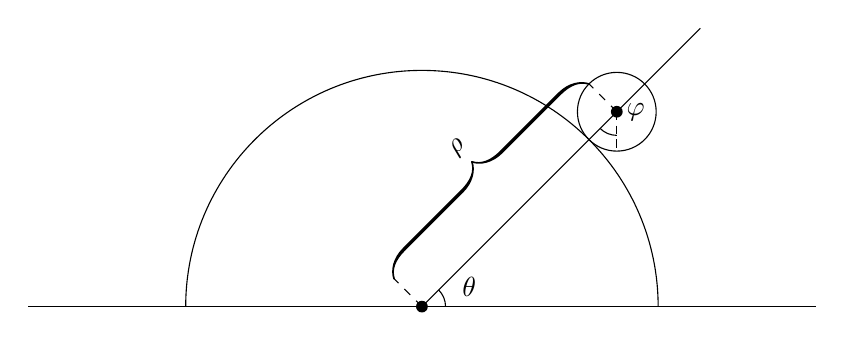
\begin{tikzpicture}
        \draw[-] (-5, 0) -- (5, 0);               % ground line
        \draw[-] (3, 0) arc (0:180:3);            % cylinder
        \draw[-] (0, 0) -- ++(45:5);              % straight line
        \draw[-] (45:3.5) circle (0.5) 
            node[circle,fill,inner sep=1.5pt] {}; % hoop
        \node at (0, 0)[circle,fill,inner sep=1.5pt] {}; % dot at bottom line
        \draw[densely dashed] (45:3.5) --++(0, -0.5);    % vertical line
        \node[above] at (0.6, 0) {$\theta$}; % theta label
        \draw[-] (0,0)+(0:0.3) arc (0:45:0.3); % theta helper line
        \node[right] at (45:3.5) {$\varphi$}; % phi label
        \draw[-] (45:3.5)+(-90:0.3) arc (-90:-135:0.3); % phi helper line 
        \draw [very thick,decorate,decoration={calligraphic brace,amplitude=10pt}] 
            (0,0)+(135:0.5) -- node[sloped,above=10pt] {$\rho$} ($ (45:3.5)+(135:0.5) $);
        \draw[dashed] (0,0)--++(135:0.5);
        \draw[dashed] (45:3.5)--++(135:0.5);
    \end{tikzpicture}
\end{figure}
Hence, we have the system 
\begin{align*}
    L &= \frac{1}{2}m(\dot{\rho}^2 + \rho^2\dot{\theta}^2)
    + \frac{1}{2}mr^2\dot{\varphi}^2 - mg\rho\sin\theta\\
    & \text{subject to}\quad \rho\geq R+r,~\rho\d\theta + r\d\varphi = 0
\end{align*}
Since we only consider the case when hoop is still on the cylinder, 
we can generalize the constraint to $\d\rho = 0$.
Using two different Lagrange's multipliers $\lambda$ and $\mu$,
we can get following set of equations
\begin{align*}
    m\ddot{\rho} - m\rho\dot{\theta}^2 + mg\sin\theta - \lambda &= 0\\
    m\rho^2\ddot{\theta} + 2m\rho\dot{\rho}\dot{\theta} + mg\rho\cos\theta
    -\rho\mu &= 0\\
    mr^2\ddot{\varphi} - r\mu &= 0
\end{align*}
Note that $\rho\d\theta + r\d\varphi = 0
\Rightarrow \dot{\rho}\dot{\theta}/r + \rho\ddot{\theta}/r + \ddot{\varphi}=0$,
substitute $\ddot{\varphi}$ into the third equation, and use the solved $\mu$, we have
\begin{align*}
    \mu &= -m\dot{\rho}\dot{\theta} - m\rho\ddot{\theta},\quad
    2m\rho^2\ddot{\theta} + 3m\rho\dot{\rho}\dot{\theta} + mg\rho\cos\theta = 0
\end{align*}
Applying $\dot{\rho}=0$ and boundary condition, we have
\begin{align*}
    \ddot{\theta} &= -\frac{g}{2\rho}\cos\theta, \quad
    \dot{\theta}\frac{\d\dot{\theta}}{\d\theta} = -\frac{g}{2\rho}\cos\theta\\
    \Rightarrow\dot{\theta}^2 &= \frac{g}{\rho}(1-\sin\theta)
\end{align*}
When the hoop is about to leave the cylinder, we should have $\lambda=0$ (and $\ddot{\rho}=0$),
then
\begin{align*}
    -m\rho\dot{\theta}^2 + mg\sin\theta &= 0\\
    2mg\sin\theta &= mg\\
    \Rightarrow\theta &= \frac{\pi}{6}
\end{align*}

\end{problem}




% \end{multicols*}
\end{document}

